\begin{pastexam}[label={px:ntu-108-esoe-ds-04}]{臺大工科海洋所 108 學年度 第 4 題}
（追蹤）

\textbf{(10 \%)} Show the sequence of swaps by which the method \textsf{bottomUpHeap} converts the
following array into a min heap. Redraw the array once for each swap.

\begin{center}
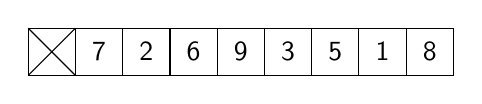
\begin{tikzpicture}[x=6mm,y=6mm]
\draw (0,0) rectangle (1,1);
\draw (0,0) -- (1,1) (0,1) -- (1,0);
\foreach \v [count=\i] in {7,2,6,9,3,5,1,8}{
  \draw (\i,0) rectangle ++(1,1);
  \node[font=\sffamily] at (\i+0.5,0.5) {\v};
}
\end{tikzpicture}
\end{center}
\end{pastexam}

\begin{pastsoln}
答案：一共交換 $4$ 次，依序是 $9 \leftrightarrow 8$、$6 \leftrightarrow 1$、$7 \leftrightarrow 1$、
$7 \leftrightarrow 5$，最後的陣列是 $\langle 1, 2, 5, 8, 3, 7, 6, 9 \rangle$。

陣列第 $0$ 格打叉，表示不用，元素放在 $A[1..8]$：節點 $i$ 的子節點是 $2i$、$2i + 1$。
\textsf{bottomUpHeap} 就是資結書第~8.2~節的由下而上建堆積（虛擬碼~8.3，這裡換成最小堆積）：從最後一個
內部節點 $\lfloor 8/2 \rfloor = 4$ 往回做到根，每個節點往下篩（sift down）——和比較小的那個子節點比，
子節點比較小就交換，一路往下直到不必交換或到了葉子。

\begin{center}
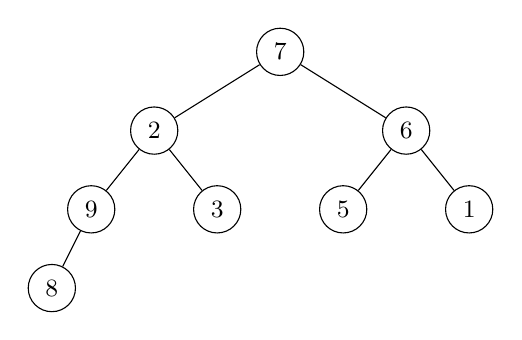
\begin{tikzpicture}[level distance=1.0cm,level 1/.style={sibling distance=3.2cm},
  level 2/.style={sibling distance=1.6cm},level 3/.style={sibling distance=1cm},
  every node/.style={circle,draw,minimum size=6mm,inner sep=0pt,font=\small}]
\node {7}
  child {node {2} child {node {9} child {node {8}} child[missing]} child {node {3}}}
  child {node {6} child {node {5}} child {node {1}}};
\end{tikzpicture}
\end{center}
上圖是一開始的陣列畫成的完全二元樹。 逐步追蹤：
\begin{itemize}
\item $i = 4$：$A[4] = 9$ 只有一個子節點 $A[8] = 8$，$9 > 8$，交換。
\item $i = 3$：$A[3] = 6$ 的子節點是 $5$、$1$，取小的 $1$；$6 > 1$，交換 $A[3]$、$A[7]$。
\item $i = 2$：$A[2] = 2$ 的子節點是 $8$、$3$，取 $3$；$2 < 3$，不交換。
\item $i = 1$：$A[1] = 7$ 的子節點是 $2$、$1$，取 $1$；$7 > 1$，交換 $A[1]$、$A[3]$。 $7$ 到了第 $3$ 格，
子節點是 $5$、$6$，取 $5$；$7 > 5$，再交換 $A[3]$、$A[6]$。 $A[6]$ 是葉子，停下。
\end{itemize}
每次交換後重畫一次陣列（第 $0$ 格不用，省略；粗體是剛交換的兩格）：
\begin{center}
\begin{tabular}{lcccccccc}
\toprule
 & $A[1]$ & $A[2]$ & $A[3]$ & $A[4]$ & $A[5]$ & $A[6]$ & $A[7]$ & $A[8]$ \\
\midrule
一開始 & 7 & 2 & 6 & 9 & 3 & 5 & 1 & 8 \\
第 1 次交換（$A[4] \leftrightarrow A[8]$） & 7 & 2 & 6 & \textbf{8} & 3 & 5 & 1 & \textbf{9} \\
第 2 次交換（$A[3] \leftrightarrow A[7]$） & 7 & 2 & \textbf{1} & 8 & 3 & 5 & \textbf{6} & 9 \\
第 3 次交換（$A[1] \leftrightarrow A[3]$） & \textbf{1} & 2 & \textbf{7} & 8 & 3 & 5 & 6 & 9 \\
第 4 次交換（$A[3] \leftrightarrow A[6]$） & 1 & 2 & \textbf{5} & 8 & 3 & \textbf{7} & 6 & 9 \\
\bottomrule
\end{tabular}
\end{center}
最後的最小堆積：
\begin{center}
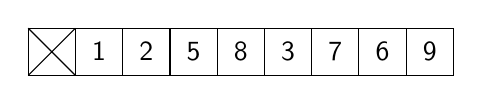
\begin{tikzpicture}[x=6mm,y=6mm]
\draw (0,0) rectangle (1,1);
\draw (0,0) -- (1,1) (0,1) -- (1,0);
\foreach \v [count=\i] in {1,2,5,8,3,7,6,9}{
  \draw (\i,0) rectangle ++(1,1);
  \node[font=\sffamily] at (\i+0.5,0.5) {\v};
}
\end{tikzpicture}
\qquad
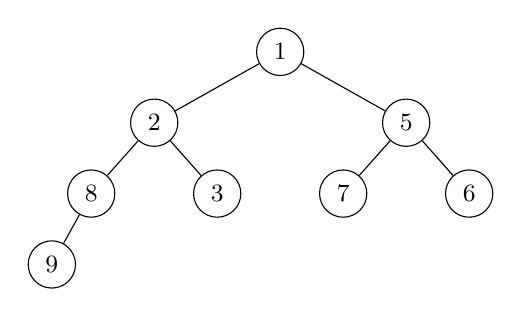
\begin{tikzpicture}[baseline=(current bounding box.center),level distance=0.9cm,level 1/.style={sibling distance=3.2cm},
  level 2/.style={sibling distance=1.6cm},level 3/.style={sibling distance=1cm},
  every node/.style={circle,draw,minimum size=6mm,inner sep=0pt,font=\small}]
\node {1}
  child {node {2} child {node {8} child {node {9}} child[missing]} child {node {3}}}
  child {node {5} child {node {7}} child {node {6}}};
\end{tikzpicture}
\end{center}
檢查：每個父節點都不大於子節點（$1 \le 2, 5$；$2 \le 8, 3$；$5 \le 7, 6$；$8 \le 9$），是最小堆積。

注意 $i = 1$ 那一步：$7$ 換到第 $3$ 格之後還比它的子節點大，要繼續往下篩，只換一次就停會得到
$\langle 1, 2, 7, 8, 3, 5, 6, 9 \rangle$，第 $3$ 格的 $7$ 大於子節點 $5$、$6$，不是堆積。 另外，由下而上建堆積
不是「一個一個插入」：依序插入 $7, 2, 6, 9, 3, 5, 1, 8$ 的交換順序和結果都不一樣，題目指定的是
\textsf{bottomUpHeap}。
\end{pastsoln}
